\chapter{Greedy Algorithms}
\section{Thinking in Greedy Algorithms}
Greedy algorithms are a class of algorithms that make the best local choice, a.k.a., {\color{blue}{greedy choice}} at each step, with the aim of approximating a {\color{blue}{global optimum}}.\\

Similar to {\color{blue}{dynamic programming}}, {\color{blue}{greedy algorithms}} are typically applied to {\color{blue}{optimization problems}}. While {\color{blue}{dynamic programming}} dynamic programming solves a problem by breaking down the problem into smaller version of the same problems,  {\color{blue}{greedy algorithms}} break down the problem into {\color{blue}{a series of consistent steps}}. At each step, it makes the {\color{blue}{greedy choice}} aiming for the {\color{blue}{local optimum}}. Although this approach does not guarantee the {\color{blue}{global optimum}}, in many cases, a greedy heuristic can efficiently approximate the global optimal solution within a reasonable amount of time.

\subsection{Relationship between DP and Greedy Algorithms}
See \hyperref[subsec:relationship_between_dp_greedy]{\ref{subsec:relationship_between_dp_greedy}: Relationship between DP and Greedy Algorithms}.

\subsection{Steps of Greedy Algorithms}
\begin{enumerate}
	\item Break down the original problem into {\color{blue}{a series of consistent steps}}.
	\item At each step, make the {\color{blue}{greedy choice}} to achieve the {\color{blue}{local optimum}}.
\end{enumerate}

\hdashrule[0.5ex]{\linewidth}{0.5pt}{1mm 3pt}
\begin{center}
{\color{magenta}{In this chapter, the greedy part of each solution will be highlighted in magenta}}.
\end{center}
\hdashrule[0.5ex]{\linewidth}{0.5pt}{1mm 3pt}

\section{LC 0767 - Reorganize String}
Given a \ul{non-empty} string {\colorbox{CodeBackground}{\lstinline|s|}}, rearrange the characters of {\colorbox{CodeBackground}{\lstinline|s|}} so that any two adjacent characters are not the same.\\

Return any possible rearrangement of {\colorbox{CodeBackground}{\lstinline|s|}} or return {\colorbox{CodeBackground}{\lstinline|""|}} if not possible.\\

Examples:
\begin{itemize}
\item {\colorbox{CodeBackground}{\lstinline|s = "aab" --> "aba"|}}
\item {\colorbox{CodeBackground}{\lstinline|s = "aaab" --> ""|}}
\end{itemize}

\subsection*{Solution - Greedy + Max Heap}
{\color{magenta}{The greedy part of this algorithm is in repeatedly picking the most frequent remaining character that doesn't match the last character placed.}}
\begin{lstlisting}
std::string reorganizeString(std::string s) {
  std::unordered_map<char, int> char2freq;
  for (char c : s) { ++char2freq[c]; }
  auto compare = [](const std::pair<char, int>& a, const std::pair<char, int>& b) {
    return a.second < b.second;
  };
  std::priority_queue<std::pair<char, int>, std::vector<std::pair<char, int>>,
                      decltype(compare)>
      max_heap(compare);
  for (const auto& pair : char2freq) {
    if (pair.second > (s.size() + 1) / 2) { return ""; }
    max_heap.emplace(pair);
  }
  std::string rearranged;
  while (max_heap.size() >= 2) {
    auto first = max_heap.top();
    max_heap.pop();
    auto second = max_heap.top();
    max_heap.pop();
    rearranged += first.first;
    rearranged += second.first;
    if (--first.second > 0) { max_heap.push(first); }
    if (--second.second > 0) { max_heap.push(second); }
  }
  if (!max_heap.empty()) { rearranged += max_heap.top().first; }
  return rearranged;
}
\end{lstlisting}

\subsection*{Solution - Greedy without Max Heap}
\begin{lstlisting}
std::string reorganizeString(std::string s) {
  std::vector<int> freq(26, 0);
  int n = s.size();
  for (char c : s) {
    ++freq[c - 'a'];
    if (freq[c - 'a'] > (n + 1) / 2) { return ""; }
  }
  std::string rearranged(n, ' ');
  for (int i = 0; i < n; ++i) {
    int max_freq = 0;
    char max_char = ' ';
    for (int j = 0; j < 26; ++j) {
      if (freq[j] > max_freq && (i == 0 || 'a' + j != rearranged[i - 1])) {
        max_freq = freq[j];
        max_char = 'a' + j;
      }
    }
    rearranged[i] = max_char;
    --freq[max_char - 'a'];
  }
  return rearranged;
}
\end{lstlisting}

\section{LC 0455 - Assign Cookies}
Assume you are an awesome parent and want to give your children some cookies of different sizes.
\begin{itemize}
	\item Each child {\colorbox{CodeBackground}{\lstinline|i|}} has a greed factor {\colorbox{CodeBackground}{\lstinline|g[i]|}}, which is the minimum size of a cookie that the child will be content with.
	\item Each cookie {\colorbox{CodeBackground}{\lstinline|j|}} has a size {\colorbox{CodeBackground}{\lstinline|s[j]|}}.
\end{itemize}
If {\colorbox{CodeBackground}{\lstinline|s[j] >= g[i]|}}, we can assign the cookie {\colorbox{CodeBackground}{\lstinline|j|}} to the child {\colorbox{CodeBackground}{\lstinline|i|}}, and the child {\colorbox{CodeBackground}{\lstinline|i|}} will be content. \\

Remember, you should give each child at most one cookie.\\

Your goal is to maximize the number of your content children and return that number.\\

Examples:
\begin{itemize}
	\item {\colorbox{CodeBackground}{\lstinline|g = [1,2,3], s = [1,1] --> 1|}}
	\item {\colorbox{CodeBackground}{\lstinline|g = [1,2], s = [1,2,3] --> 2|}}
\end{itemize}

\subsection*{Solution 1 - Greedy}
\begin{itemize}
	\item Design Steps - At each step, assign a cookie to a child until all cookies are distributed or each child has a cookie.
	\item Greedy Choice - {\color{magenta}{At each step, try to use the largest cookies left to satisfy the child with the biggest greedy factor.}}
	\item Global Optimum - Maximum content children.
\end{itemize}
\begin{lstlisting}
int findContentChildren(std::vector<int>& g, std::vector<int>& s) {
  std::sort(g.begin(), g.end(), std::greater<int>());
  std::sort(s.begin(), s.end(), std::greater<int>());
  // assign the biggest cookie to the child with the biggest greed factor
  // i - idx of child
  // j - idx of cookie
  int j = 0;
  for (int i = 0; i < g.size(); ++i) {
    if (j < s.size() && s[j] >= g[i]) { ++j; }
  }
  return j;
}
\end{lstlisting}

\subsection*{Solution 2 - Greedy}
\begin{itemize}
	\item Design Steps - At each step, assign a cookie to a child until all cookies are distributed or each child has a cookie.
	\item Greedy Choice - {\color{magenta}{At each step, try to use the smallest cookies left to satisfy the child with the smallest greedy factor.}}
	\item Global Optimum - Maximum content children.
\end{itemize}
\begin{lstlisting}
int findContentChildren(std::vector<int>& g, std::vector<int>& s) {
  std::sort(g.begin(), g.end());
  std::sort(s.begin(), s.end());
  // assign the smallest cookie to the child with the smallest greed factor
  // i - idx of child
  // j - idx of cookie
  int i = 0;
  for (int j = 0; j < s.size(); ++j) {
    if (i < g.size() && s[j] >= g[i]) { ++i; }
  }
  return i;
}
\end{lstlisting}

\section{LC 0860 - Lemonade Change}
At a lemonade stand, each lemonade costs {\colorbox{CodeBackground}{\lstinline|$5|}}. Customers are standing in a queue to buy from you and order one at a time (in the order specified by {\colorbox{CodeBackground}{\lstinline|bills|}}). Each customer will only buy one lemonade and pay with either a {\colorbox{CodeBackground}{\lstinline|$5|}}, {\colorbox{CodeBackground}{\lstinline|$10|}}, or {\colorbox{CodeBackground}{\lstinline|$20|}} bill. You must provide the correct change to each customer so that the net transaction is that the customer pays {\colorbox{CodeBackground}{\lstinline|$5|}}.\\

Note that you do not have any change in hand at first.\\

Given a \ul{non-empty} integer array {\colorbox{CodeBackground}{\lstinline|bills|}} where {\colorbox{CodeBackground}{\lstinline|bills[i]|}} is the bill the {\colorbox{CodeBackground}{\lstinline|i|}}th customer pays, return {\colorbox{CodeBackground}{\lstinline|true|}} if you can provide every customer with the correct change, or {\colorbox{CodeBackground}{\lstinline|false|}} otherwise.\\

Examples:
\begin{itemize}
	\item {\colorbox{CodeBackground}{\lstinline|bills = [5,5,5,10,20] --> true|}}
	\item {\colorbox{CodeBackground}{\lstinline|bills = [5,5,10,10,20] --> false|}}
\end{itemize}

\subsection*{Solution - Greedy}
\begin{itemize}
\item If it's a {\colorbox{CodeBackground}{\lstinline|$5|}} bill, no change is needed -- just add it to the cash on hand.
\item If it's a {\colorbox{CodeBackground}{\lstinline|$10|}} bill, give back one {\colorbox{CodeBackground}{\lstinline|$5|}} bill if available. If you can't, there's no way to continue, return {\colorbox{CodeBackground}{\lstinline|false|}}.
\item {\color{magenta}{If it's a {\colorbox{CodeBackground}{\lstinline|$20|}} bill, always prefer to give back {\colorbox{CodeBackground}{\lstinline|$10|}}, then give back {\colorbox{CodeBackground}{\lstinline|$5|}}.}} If neither option is available, return {\colorbox{CodeBackground}{\lstinline|false|}}.
\end{itemize}
\begin{lstlisting}
bool lemonadeChange(std::vector<int>& bills) {
  int ten = 0;
  int five = 0;
  for (int bill : bills) {
    if (bill == 5) {
      five++;
    } else if (bill == 10) {
      if (five == 0) { return false; }
      five--;
      ten++;
    } else if (bill == 20) {
      if (ten > 0 && five > 0) {
        ten--;
        five--;
      } else if (five >= 3) {
        five -= 3;
      } else {
        return false;
      }
    }
  }
  return true;
}
\end{lstlisting}

\section{LC 0055 - Jump Game}\label{lc0055}
You are given a {\colorbox{CodeBackground}{\lstinline|0|}}-indexed array of integers {\colorbox{CodeBackground}{\lstinline|nums|}} of length {\colorbox{CodeBackground}{\lstinline|n|}} ({\colorbox{CodeBackground}{\lstinline|n >= 1|}}). You are initially positioned at {\colorbox{CodeBackground}{\lstinline|nums[0]|}}. \\

Each element {\colorbox{CodeBackground}{\lstinline|nums[i]|}} represents the maximum length of a forward jump from index {\colorbox{CodeBackground}{\lstinline|i|}}. In other words, if you are at {\colorbox{CodeBackground}{\lstinline|nums[i]|}}, you can jump to any {\colorbox{CodeBackground}{\lstinline|nums[i + j]|}} where:
\begin{itemize}
	\item {\colorbox{CodeBackground}{\lstinline|0 <= j <= nums[i]|}}
	\item {\colorbox{CodeBackground}{\lstinline|i + j < n|}}
\end{itemize}

Return {\colorbox{CodeBackground}{\lstinline|true|}} if you can reach the last index, or {\colorbox{CodeBackground}{\lstinline|false|}} otherwise.\\

Examples:
\begin{itemize}
	\item {\colorbox{CodeBackground}{\lstinline|[2,3,1,1,4] --> True|}}
	\item {\colorbox{CodeBackground}{\lstinline|[3,2,1,0,4] --> False|}}
\end{itemize}

\subsection*{Solution - Greedy}\label{solution:lc0055_greedy}
\begin{itemize}
	\item Design Steps - At each step, make a single jump at the corresponding position.
	\item Greedy Choice - {\color{magenta}{At each step, jump to the furthest possible distance.}}
	\item Global Optima - Maximum distance possible through jumping.
\end{itemize}
\begin{lstlisting}
bool canJump(std::vector<int>& nums) {
	int max_reach = 0;
	for (int i = 0; i < nums.size(); ++i) {
		if (max_reach < i) { return false; }
		max_reach = std::max(max_reach, i + nums[i]);
	}
	return true;
}
\end{lstlisting}

\subsection*{Other Solutions}
\begin{itemize}
	\item \hyperref[solution:lc0055_dp]{DP (Time Limit Exceeded)}
	%	\item \hyperref[solution:lc0055_greedy]{Greedy}
\end{itemize}

\subsection*{Related}
\begin{itemize}
	\item \hyperref[lc0055]{LC 0055 - Jump Game}
	\item \hyperref[lc0045]{LC 0045 - Jump Game II}
\end{itemize}

\section{LC 0045 - Jump Game II}\label{lc0045}
You are given a {\colorbox{CodeBackground}{\lstinline|0|}}-indexed array of integers {\colorbox{CodeBackground}{\lstinline|nums|}} of length {\colorbox{CodeBackground}{\lstinline|n|}} ({\colorbox{CodeBackground}{\lstinline|n >= 1|}}). You are initially positioned at {\colorbox{CodeBackground}{\lstinline|nums[0]|}}. \\

Each element {\colorbox{CodeBackground}{\lstinline|nums[i]|}} represents the maximum length of a forward jump from index {\colorbox{CodeBackground}{\lstinline|i|}}. In other words, if you are at {\colorbox{CodeBackground}{\lstinline|nums[i]|}}, you can jump to any {\colorbox{CodeBackground}{\lstinline|nums[i + j]|}} where:
\begin{itemize}
	\item {\colorbox{CodeBackground}{\lstinline|0 <= j <= nums[i]|}}
	\item {\colorbox{CodeBackground}{\lstinline|i + j < n|}}
\end{itemize}

Return the minimum number of jumps to reach {\colorbox{CodeBackground}{\lstinline|nums[n - 1]|}}. \ul{It's guaranteed that you can reach {\colorbox{CodeBackground}{\lstinline|nums[n - 1]|}}.}\\

Examples:
\begin{itemize}
	\item {\colorbox{CodeBackground}{\lstinline|[2,3,1,1,4] --> 2 (2-->3-->4)|}}
	\item {\colorbox{CodeBackground}{\lstinline|[2,3,0,1,4] --> 2 (2-->3-->4)|}}
\end{itemize}

\subsection*{Solution - Greedy}\label{solution:lc0045_greedy}
\begin{lstlisting}
int jump(std::vector<int>& nums) {
  // edge case
  if (nums.size() == 1) { return 0; }
  int num_jumps = 0;
  int cur_reach = 0;
  int next_reach = 0;
  for (int i = 0; i < nums.size(); ++i) {
    next_reach = std::max(next_reach, i + nums[i]);
    // when we reach the end of the current jump range, we need to make another jump
    if (i == cur_reach) {
      ++num_jumps;
      cur_reach = next_reach;
      if (cur_reach >= nums.size() - 1) { break; }
    }
  }
  return num_jumps;
}
\end{lstlisting}

\subsection*{Solution - Greedy, Optimized}
\begin{lstlisting}
int jump(std::vector<int>& nums) {
  // edge case
  if (nums.size() == 1) { return 0; }
  int num_jumps = 0;
  int cur_reach = 0;
  int next_reach = 0;
  for (int i = 0; i < nums.size() - 1; ++i) {
    next_reach = std::max(next_reach, i + nums[i]);
    // when we reach the end of the current jump range, we need to make another jump
    if (i == cur_reach) {
      ++num_jumps;
      cur_reach = next_reach;
    }
  }
  return num_jumps;
}
\end{lstlisting}

\subsection*{Other Solutions}
\begin{itemize}
	\item \hyperref[solution:lc0045_dp]{DP}
%	\item \hyperref[solution:lc0045_greedy]{Greedy}
\end{itemize}

\subsection*{Related}
\begin{itemize}
	\item \hyperref[lc0055]{LC 0055 - Jump Game}
	\item \hyperref[lc0045]{LC 0045 - Jump Game II}
\end{itemize}

\section{LC 0121 - Best Time to Buy and Sell Stock}\label{lc0121}
You are given a \ul{non-empty} array {\colorbox{CodeBackground}{\lstinline|prices|}} where {\colorbox{CodeBackground}{\lstinline|prices[i]|}} is the price of a given stock on the {\colorbox{CodeBackground}{\lstinline|i|}}th day.\\

You want to maximize your profit by choosing \ul{a single day} to buy one stock and choosing \ul{a different day in the future} to sell that stock.\\

Return the \ul{maximum profit} you can achieve from this transaction. If you cannot achieve any profit, return {\colorbox{CodeBackground}{\lstinline|0|}}.\\

Examples:
\begin{itemize}
	\item {\colorbox{CodeBackground}{\lstinline|prices = [7,1,5,3,6,4] --> 5|}}
	\item {\colorbox{CodeBackground}{\lstinline|prices = [7,6,4,3,1] --> 0|}}
\end{itemize}

\subsection*{Solution - Greedy}\label{solution:lc0121_greedy}
On each day:
\begin{enumerate}
\item Track the lowest stock price so far.
\item {\color{magenta}{Try to sell the stock to see whether we can achieve a higher profit.}}
\end{enumerate}
\begin{lstlisting}
int maxProfit(std::vector<int>& prices) {
	int max_profit = 0;
	int min_price = std::numeric_limits<int>::max();
	for (int price : prices) {
		// if the current price is less than min_price, update min_price
		if (price < min_price) { min_price = price; }
		// if selling on this day would give us a higher profit than before, update max_profit
		if (price - min_price > max_profit) { max_profit = price - min_price; }
	}
	return max_profit;
}
\end{lstlisting}

\subsection*{Solution - Greedy, Optimized}
\begin{lstlisting}
int maxProfit(std::vector<int>& prices) {
	int max_profit = 0;
	int min_price = std::numeric_limits<int>::max();
	for (int price : prices) {
		if (price < min_price) {
			// if the current price is less than min_price, update min_price
			min_price = price;
		} else if (price - min_price > max_profit) {
			// if selling on this day would give us a higher profit than before, update max_profit
			max_profit = price - min_price;
		}
	}
	return max_profit;
}
\end{lstlisting}

\subsection*{Other Solutions}
\begin{itemize}
%\item \hyperref[solution:lc0121_greedy]{Greedy}
\item \hyperref[solution:lc0121_dp]{DP}
\end{itemize}

\subsection*{Related}
\begin{itemize}
	\item \hyperref[lc0121]{LC 0121 - Best Time to Buy and Sell Stock}
	\item \hyperref[lc0122]{LC 0122 - Best Time to Buy and Sell Stock II}
	\item \hyperref[lc0123]{LC 0123 - Best Time to Buy and Sell Stock III}
	\item \hyperref[lc0188]{LC 0188 - Best Time to Buy and Sell Stock IV}
\end{itemize}

\section{LC 0122 - Best Time to Buy and Sell Stock II}\label{lc0122}
You are given a \ul{non-empty} array {\colorbox{CodeBackground}{\lstinline|prices|}} where {\colorbox{CodeBackground}{\lstinline|prices[i]|}} is the price of a given stock on the {\colorbox{CodeBackground}{\lstinline|i|}}th day.\\

On each day, you may decide to buy and/or sell the stock. You can only hold \ul{at most one share of the stock at any time}. However, you can buy it then immediately sell it on the same day.\\

Find and return the \ul{maximum profit} you can achieve.\\

Examples:
\begin{itemize}
	\item {\colorbox{CodeBackground}{\lstinline|prices = [7,1,5,3,6,4] --> 7|}}
	\item {\colorbox{CodeBackground}{\lstinline|prices = [1,2,3,4,5] --> 4|}}
	\item {\colorbox{CodeBackground}{\lstinline|prices = [7,6,4,3,1] --> 0|}}
\end{itemize}

\subsection*{Solution - Greedy}\label{solution:lc0122_greedy}
On each day:
\begin{enumerate}
\item {\color{magenta}{Whenever you find a chance to make a profit (the price tomorrow is higher than the price today), buy today and sell tomorrow.}}
\item Keep a running total of these profits.
\end{enumerate}
\begin{lstlisting}
int maxProfit(std::vector<int>& prices) {
	int profit = 0;
	for (int i = 0; i < prices.size() - 1; ++i) {
		// if the next day's price is higher than today's, we buy today and sell tomorrow
		if (prices[i + 1] > prices[i]) { profit += prices[i + 1] - prices[i]; }
	}
	return profit;
}
\end{lstlisting}

\subsection*{Other Solutions}
\begin{itemize}
%\item \hyperref[solution:lc0122_greedy]{Greedy}
\item \hyperref[solution:lc0122_dp]{DP}
\end{itemize}

\subsection*{Related}
\begin{itemize}
	\item \hyperref[lc0121]{LC 0121 - Best Time to Buy and Sell Stock}
	\item \hyperref[lc0122]{LC 0122 - Best Time to Buy and Sell Stock II}
	\item \hyperref[lc0123]{LC 0123 - Best Time to Buy and Sell Stock III}
	\item \hyperref[lc0188]{LC 0188 - Best Time to Buy and Sell Stock IV}
\end{itemize}

\section{LC 0053 - Maximum Sum of Subarray}
Given an \ul{non-empty} integer array {\colorbox{CodeBackground}{\lstinline|nums|}}, find the {\colorbox{CodeBackground}{\lstinline|subarray|}} with the largest sum, and return its sum.\\

Examples:
\begin{itemize}
	\item {\colorbox{CodeBackground}{\lstinline|nums = [-2,1,-3,4,-1,2,1,-5,4] --> 6 ([4,-1,2,1])|}}
	\item {\colorbox{CodeBackground}{\lstinline|nums = [1] --> 1|}}
	\item {\colorbox{CodeBackground}{\lstinline|nums = [5,4,-1,7,8] --> 23 ([5,4,-1,7,8])|}}
\end{itemize}

\subsection*{Solution - Greedy}\label{solution:lc0053_greedy}
\begin{enumerate}
\item Start with the first element and calculate the sum of the subarray as you go.
\item {\color{magenta}{If the sum of the current subarray is negative, we start a new subarray from the next element.}}
\item Track the subarray which achieves the maximum sum.
\end{enumerate}


\begin{lstlisting}
int maxSubArray(std::vector<int>& nums) {
  int max_sum = std::numeric_limits<int>::min();
  int sum = 0;
  for (int i = 0; i < nums.size(); ++i) {
    sum += nums[i];
    max_sum = std::max(max_sum, sum);
    if (sum <= 0) { sum = 0; }
  }
  return max_sum;
}
\end{lstlisting}

\subsection*{Other Solutions}
\begin{itemize}
%\item \hyperref[solution:lc0053_greedy]{Greedy}
\item \hyperref[solution:lc0053_dp]{DP}
\end{itemize}

\section{LC 1005 - Maximize Sum of Array after K Negations}
Given an \ul{non-empty} integer array {\colorbox{CodeBackground}{\lstinline|nums|}} and an integer {\colorbox{CodeBackground}{\lstinline|k|}} ({\colorbox{CodeBackground}{\lstinline|k >= 1|}}), modify the array in the following way: choose an index {\colorbox{CodeBackground}{\lstinline|i|}} and replace {\colorbox{CodeBackground}{\lstinline|nums[i]|}} with {\colorbox{CodeBackground}{\lstinline|-nums[i]|}}. \\

You should apply this process exactly {\colorbox{CodeBackground}{\lstinline|k|}} times, and you may choose the same index {\colorbox{CodeBackground}{\lstinline|i|}} multiple times.\\

Return the largest possible sum of the array after modifying it in this way.\\

Examples:
\begin{itemize}
\item {\colorbox{CodeBackground}{\lstinline|nums = [4,2,3], k = 1 --> 5|}}\\
Choose index {\colorbox{CodeBackground}{\lstinline|1|}} and nums becomes {\colorbox{CodeBackground}{\lstinline|[4,-2,3]|}}.
\item {\colorbox{CodeBackground}{\lstinline|nums = [3,-1,0,2], k = 3 --> 6|}}\\
Choose indices {\colorbox{CodeBackground}{\lstinline|(1, 2, 2)|}} and nums becomes {\colorbox{CodeBackground}{\lstinline|[3,1,0,2]|}}.
\item {\colorbox{CodeBackground}{\lstinline|nums = [2,-3,-1,5,-4], k = 2 --> 13|}}\\
Choose indices {\colorbox{CodeBackground}{\lstinline|(1, 4)|}} and nums becomes {\colorbox{CodeBackground}{\lstinline|[2,3,-1,5,4]|}}.
\end{itemize}

\subsection*{Solution - Greedy}
\begin{enumerate}
\item Sort the {\colorbox{CodeBackground}{\lstinline|nums|}} in ascending order.
\item {\color{magenta}{Flip the negative numbers from the most negative to the least negative}} until we run out of {\colorbox{CodeBackground}{\lstinline|k|}} or negative numbers.
\item If we still have some {\colorbox{CodeBackground}{\lstinline|k|}} left after all negatives have been flipped, then:
  \subitem - If {\colorbox{CodeBackground}{\lstinline|k|}} is even, we're done, because flipping any number twice will bring it back to its original value.
  \subitem - If {\colorbox{CodeBackground}{\lstinline|k|}} is odd, {\color{magenta}{flip the smallest positive number}}.
\end{enumerate}
\begin{lstlisting}
int largestSumAfterKNegations(std::vector<int>& nums, int k) {
  std::sort(nums.begin(), nums.end());
  for (int i = 0; i < nums.size(); ++i) {
    if (nums[i] < 0 && k > 0) {
      nums[i] *= -1;
      --k;
    }
  }
  if (k % 2 == 1) { *std::min_element(nums.begin(), nums.end()) *= -1; }
  return std::accumulate(nums.begin(), nums.end(), 0);
}
\end{lstlisting}

\section{LC 0011 - Container With Most Water}\label{lc0011}
There are {\colorbox{CodeBackground}{\lstinline|n|}} ({\colorbox{CodeBackground}{\lstinline|n >= 2|}}) vertical lines drawn and the {\colorbox{CodeBackground}{\lstinline|i|}}th line is of the height {\colorbox{CodeBackground}{\lstinline|height[i]|}}. Find two lines that together with the x-axis form a container to store water. Return the maximum amount of water a container can store.\\

For example: {\colorbox{CodeBackground}{\lstinline|height = [1,8,6,2,5,4,8,3,7] --> 49 (7 x 7)|}}
\begin{figure}[H]
	\centering
	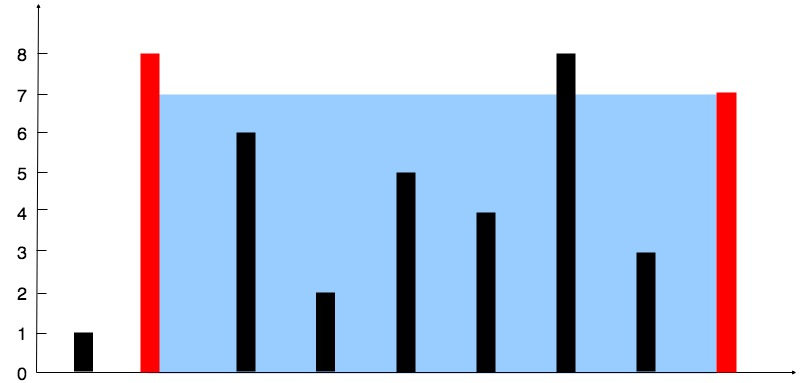
\includegraphics[width=0.5\linewidth]{images/lc0011_example}
	\label{fig:lc0011example}
\end{figure}

\subsection*{Solution - Greedy}
\begin{itemize}
	\item Design Steps - Begin with {\colorbox{CodeBackground}{\lstinline|left|}} and {\colorbox{CodeBackground}{\lstinline|right|}} pointers on two sides. At each step, move one pointer inward to search the largest container until the two pointers meet.
	\item Greedy Choice - {\color{magenta}{At each step, move the pointer of the shorter line inward.}} This is the only way we might get a larger container next step, because: 1) the water width is fixed at the next step, which is the current width minus $1$ 2) the height of the container is limited by the shorter line.
	\item Global Optimum - The largest container.
\end{itemize}
\begin{lstlisting}
int maxArea(std::vector<int>& height) {
	int max_water = 0;
	int left = 0;
	int right = height.size() - 1;
	while (left < right) {
		int water_height = std::min(height[left], height[right]);
		int water_width = right - left;
		max_water = std::max(max_water, water_height * water_width);
		// move the pointer of the shorter line inward
		if (height[left] < height[right]) {
			left++;
		} else {
			right--;
		}
	}
	return max_water;
}
\end{lstlisting}

\subsection*{Related - Two Pointers + Inward Search}
\begin{itemize}
\item \hyperref[lc0011]{LC 0011 - Container With Most Water}
\item \hyperref[lc0167]{LC 0167 - Two Sum II - Input Array Is Sorted}
\item \hyperref[lc0015]{LC 0015 - 3Sum}
\item \hyperref[lc0018]{LC 0018 - 4Sum}
\end{itemize}

\section{LC 0134 - Gas Station}
There are {\colorbox{CodeBackground}{\lstinline|n|}} ({\colorbox{CodeBackground}{\lstinline|n >= 1|}}) gas stations along a \ul{circular route}, where the amount of gas at the {\colorbox{CodeBackground}{\lstinline|i|}}th station is {\colorbox{CodeBackground}{\lstinline|gas[i]|}}.\\

You have a car with an \ul{unlimited gas tank} and it costs {\colorbox{CodeBackground}{\lstinline|cost[i]|}} of gas to travel from the {\colorbox{CodeBackground}{\lstinline|i|}}th station to its next {\colorbox{CodeBackground}{\lstinline|(i+1)|}}th station. You begin the journey with an empty tank at one of the gas stations.\\

Given two integer arrays {\colorbox{CodeBackground}{\lstinline|gas|}} and {\colorbox{CodeBackground}{\lstinline|cost|}}, return the \ul{starting gas station's index} if you can travel around the circuit once in the \ul{clockwise direction}, otherwise return {\colorbox{CodeBackground}{\lstinline|-1|}}. If there exists a solution, it is guaranteed to be unique.\\

Examples:
\begin{itemize}
	\item {\colorbox{CodeBackground}{\lstinline|gas = [1,2,3,4,5], cost = [3,4,5,1,2] --> 3|}}
	\item {\colorbox{CodeBackground}{\lstinline|gas = [2,3,4], cost = [3,4,3] --> -1|}}
\end{itemize}

\subsection*{Solution - Greedy}
\begin{enumerate}
\item Start at station {\colorbox{CodeBackground}{\lstinline|0|}} and attempt to travel to each station.
\item Keep track of both the total amount gas ({\colorbox{CodeBackground}{\lstinline|total_gas|}}) and the gas you currently have as you travel ({\colorbox{CodeBackground}{\lstinline|cur_tank|}}).
\item {\color{magenta}{If you ever run out of gas before reaching the next station, consider that station as a new starting point.}}
\item At the end, if the total amount of gas ({\colorbox{CodeBackground}{\lstinline|total_gas|}}) is non-negative, the journey can be completed, and we return the starting station. Otherwise, we return {\colorbox{CodeBackground}{\lstinline|-1|}}.
\end{enumerate}

\begin{lstlisting}
int canCompleteCircuit(std::vector<int>& gas, std::vector<int>& cost) {
  int total_gas = 0;
  int cur_tank = 0;
  int start_station = 0;
  for (int i = 0; i < gas.size(); ++i) {
    total_gas += gas[i] - cost[i];
    cur_tank += gas[i] - cost[i];
    if (cur_tank < 0) {
      start_station = i + 1;
      cur_tank = 0;
    }
  }
  return (total_gas >= 0) ? start_station : -1;
}
\end{lstlisting}

\section{LC 0135 - Candy}
There are {\colorbox{CodeBackground}{\lstinline|n|}} ({\colorbox{CodeBackground}{\lstinline|n >= 1|}}) children standing in a line. Each child is assigned a \ul{rating value} given in the integer array {\colorbox{CodeBackground}{\lstinline|ratings|}}.\\

You are giving candies to these children subjected to the following requirements:
\begin{itemize}
	\item Each child must have at least one candy.
	\item Children with a higher \ul{rating value} get more candies than their neighbors.
\end{itemize}

Return the minimum number of candies you need to have to distribute the candies to the children.\\

Examples:
\begin{itemize}
\item {\colorbox{CodeBackground}{\lstinline|ratings = [1,0,2] --> 5|}}\\
You can allocate to the first, second and third child with 2, 1, 2 candies respectively.
\item {\colorbox{CodeBackground}{\lstinline|ratings = [1,2,2] --> 4|}}\\
You can allocate to the first, second and third child with 1, 2, 1 candies respectively. The third child gets 1 candy because it satisfies the above two conditions.
\end{itemize}

\subsection*{Solution - Greedy}
\begin{enumerate}
\item We give each child {\colorbox{CodeBackground}{\lstinline|1|}} candy to start with.
\item We make a first pass from \ul{left to right}. {\color{magenta}{For each child (except the first one), if their rating is higher than the previous child, we give them one more candy than the previous child.}}
\item We make a second pass from \ul{right to left}. {\color{magenta}{For each child (except the last one), if their rating is higher than the next child, we check if the current candy count satisfies the condition. If not, we update the count to be one more than the next child's count.}}
\item The sum of the candies after the second pass will give us the minimum candies required.
\end{enumerate}
\begin{lstlisting}
int candy(std::vector<int>& ratings) {
  int n = ratings.size();
  if (n <= 1) { return n; }
  std::vector<int> candy(n, 1);
  for (int i = 1; i < n; ++i) {
    if (ratings[i] > ratings[i - 1]) { candy[i] = candy[i - 1] + 1; }
  }
  for (int i = n - 2; i >= 0; --i) {
    if (ratings[i] > ratings[i + 1]) { candy[i] = std::max(candy[i], candy[i + 1] + 1); }
  }
  return std::accumulate(candy.begin(), candy.end(), 0);
}
\end{lstlisting}

\section{LC 0056 - Merge Intervals}\label{lc0056}
\hyperref[sec:interval_range]{[Interval \& Range]}\\

Given an \ul{non-empty} array of {\colorbox{CodeBackground}{\lstinline|intervals|}} where {\colorbox{CodeBackground}{\lstinline|intervals[i] = [start_i, end_i]|}}, merge all overlapping intervals, and return an array of the non-overlapping intervals that cover all the intervals in the input.\\

Examples:
\begin{itemize}
	\item {\colorbox{CodeBackground}{\lstinline|intervals = [[1,3],[2,6],[8,10],[15,18]] --> [[1,6],[8,10],[15,18]]|}}
	\item {\colorbox{CodeBackground}{\lstinline|intervals = [[1,4],[4,5]] --> [[1,5]]|}}
\end{itemize}

\subsection*{Solution - Greedy, Sort By Start}
\begin{enumerate}
\item Sort the intervals by their starting points ({\colorbox{CodeBackground}{\lstinline|start_i|}}) in ascending order.
\item For each interval:
  \subitem - {\color{magenta}{If the current interval does not overlap with the previous one, simply add the current interval.}}
  \subitem - {\color{magenta}{If there is an overlap, merge the current interval with the previous one.}}
\end{enumerate}
\begin{lstlisting}
std::vector<std::vector<int>> merge(std::vector<std::vector<int>>& intervals) {
  std::sort(intervals.begin(), intervals.end(),
            [](const std::vector<int>& lhs, const std::vector<int>& rhs) {
              return lhs[0] < rhs[0];
            });
  std::vector<std::vector<int>> merged;
  for (const auto& interval : intervals) {
    if (!merged.empty() && interval[0] <= merged.back()[1]) {
      merged.back()[1] = std::max(merged.back()[1], interval[1]);
    } else {
      merged.push_back(interval);
    }
  }
  return merged;
}
\end{lstlisting}

\section{LC 0495 - Teemo Attacking}\label{lc0495}
\hyperref[sec:interval_range]{[Interval \& Range]}\\

Our hero Teemo is attacking an enemy Ashe with poison attacks! When Teemo attacks Ashe, Ashe gets poisoned for a exactly {\colorbox{CodeBackground}{\lstinline|duration|}} seconds. More formally, an attack at second {\colorbox{CodeBackground}{\lstinline|t|}} will mean Ashe is poisoned during the inclusive time interval {\colorbox{CodeBackground}{\lstinline|[t, t + duration - 1]|}}. If Teemo attacks again before the poison effect ends, the timer for it is reset, and the poison effect will end {\colorbox{CodeBackground}{\lstinline|duration|}} seconds after the new attack.\\

You are given a \ul{non-empty} \ul{non-decreasing} integer array {\colorbox{CodeBackground}{\lstinline|attacks|}}, where {\colorbox{CodeBackground}{\lstinline|attacks[i]|}} denotes that Teemo attacks Ashe at second {\colorbox{CodeBackground}{\lstinline|attacks[i]|}}, and an integer {\colorbox{CodeBackground}{\lstinline|duration|}}.\\

Return the total number of seconds that Ashe is poisoned.\\

Examples:
\begin{itemize}
\item {\colorbox{CodeBackground}{\lstinline|attacks = [1,4], duration = 2 --> 4|}}
\item {\colorbox{CodeBackground}{\lstinline|attacks = [1,2], duration = 2 --> 3|}}
\end{itemize}

\subsection*{Solution - Greedy}
\begin{lstlisting}
int findPoisonedDuration(std::vector<int>& attacks, int duration) {
  int total_duration = 0;
  for (int i = 0; i < attacks.size() - 1; ++i) {
    int diff = attacks[i + 1] - attacks[i];
    total_duration += std::min(diff, duration);
  }
  total_duration += duration;
  return total_duration;
}
\end{lstlisting}

\subsection*{Solution 2 - Interval Merge}
\begin{lstlisting}
int findPoisonedDuration(std::vector<int>& attacks, int duration) {
  std::vector<std::vector<int>> intervals;
  for (int attack : attacks) { intervals.push_back({attack, attack + duration - 1}); }
  std::vector<std::vector<int>> merged;
  for (const auto& interval : intervals) {
    if (!merged.empty() && interval[0] <= merged.back()[1]) {
      merged.back()[1] = std::max(merged.back()[1], interval[1]);
    } else {
      merged.push_back(interval);
    }
  }
  int total_duration = 0;
  for (const auto& interval : merged) { total_duration += interval[1] - interval[0] + 1; }
  return total_duration;
}
\end{lstlisting}

\section{LC 0616 - Add Bold Tag in String}\label{lc0616}
\hyperref[sec:interval_range]{[Interval \& Range]}\\

You are given a \ul{non-empty} string {\colorbox{CodeBackground}{\lstinline|s|}} and an array of strings {\colorbox{CodeBackground}{\lstinline|words|}}.\\

You should add a closed pair of bold tag {\colorbox{CodeBackground}{\lstinline|<b>|}} and {\colorbox{CodeBackground}{\lstinline|</b>|}} to wrap the substrings in {\colorbox{CodeBackground}{\lstinline|s|}} that exist in {\colorbox{CodeBackground}{\lstinline|words|}}.

\begin{itemize}
\item If two such substrings overlap, you should wrap them together with only one pair of closed bold-tag.
\item If two substrings wrapped by bold tags are consecutive, you should combine them.
\end{itemize}

Return {\colorbox{CodeBackground}{\lstinline|s|}} after adding the bold tags.\\

\begin{itemize}
\item {\colorbox{CodeBackground}{\lstinline|s = "abcxyz123", words = ["abc","123"] --> "<b>abc</b>xyz<b>123</b>"|}}
\item {\colorbox{CodeBackground}{\lstinline|s = "aaabbb", words = ["aa","b"] --> "<b>aaabbb</b>"|}}
\end{itemize}

\subsection*{Solution - Interval Merge}
\begin{lstlisting}
std::string addBoldTag(std::string s, std::vector<std::string>& words) {
  std::vector<std::pair<int, int>> intervals;
  // 1. create intervals for all words
  for (const std::string& word : words) {
    size_t pos = s.find(word);
    while (pos != std::string::npos) {
      intervals.emplace_back(pos, pos + word.size());
      pos = s.find(word, pos + 1);
    }
  }
  // 2. merge intervals
  std::vector<std::pair<int, int>> merged;
  std::sort(intervals.begin(), intervals.end(),
            [](const auto& lhs, const auto& rhs) { return lhs.first < rhs.first; });
  for (const auto& interval : intervals) {
    if (!merged.empty() && interval.first <= merged.back().second) {
      merged.back().second = std::max(merged.back().second, interval.second);
    } else {
      merged.push_back(interval);
    }
  }
  // add bold tags
  std::string result;
  size_t i = 0;
  for (const auto& interval : merged) {
    result += s.substr(i, interval.first - i);
    result += "<b>";
    result += s.substr(interval.first, interval.second - interval.first);
    result += "</b>";
    i = interval.second;
  }
  result += s.substr(i);
  return result;
}
\end{lstlisting}

\section{LC 0253 - Meeting Rooms II}\label{lc0253}
\hyperref[sec:interval_range]{[Interval \& Range]}\\

Given a \ul{non-empty} array of meeting time {\colorbox{CodeBackground}{\lstinline|intervals|}} intervals where {\colorbox{CodeBackground}{\lstinline|intervals[i] = [start_i, end_i]|}}, return the minimum number of conference rooms required. (Hint: If meeting A and meeting B overlap, two rooms are needed to host the two meetings simultaneously.) \\

Examples:
\begin{itemize}
\item {\colorbox{CodeBackground}{\lstinline|intervals = [[0,30],[5,10],[15,20]] --> 2|}}
\item {\colorbox{CodeBackground}{\lstinline|intervals = [[7,10],[2,4]] --> 1|}}
\end{itemize}

\subsection*{Solution - Greedy + Priority Queue}
\begin{enumerate}
\item Sort the intervals by their start times.
\item Use a \ul{min heap} to keep track of the end times of the meetings currently occupying the rooms.
\item {\color{magenta}{Every time we consider a new meeting, we'll look at the \ul{min heap} to see if the earliest meeting has ended.}}
  \subitem {\color{magenta}{- If the new meeting starts after the top in the heap ends, we can use that room.}}
  \subitem - {\color{magenta}{If not, we need a new room.}}
\end{enumerate}
Note that we sort meetings by start times because we are simulating the process of occupying rooms.
\begin{lstlisting}
int minMeetingRooms(std::vector<std::vector<int>>& intervals) {
  std::sort(intervals.begin(), intervals.end(),
            [](const std::vector<int>& lhs, const std::vector<int>& rhs) {
              return lhs[0] < rhs[0];
            });
  std::priority_queue<int, std::vector<int>, std::greater<int>> min_heap;
  min_heap.push(intervals[0][1]);
  for (int i = 1; i < intervals.size(); ++i) {
    if (intervals[i][0] >= min_heap.top()) { min_heap.pop(); }
    min_heap.push(intervals[i][1]);
  }
  return min_heap.size();
}
\end{lstlisting}

\subsection*{Related}
\begin{itemize}
\item \hyperref[lc0252]{LC 0252 - Meeting Rooms}
\item \hyperref[lc0253]{LC 0253 - Meeting Rooms II}
\end{itemize}

\section{LC 0435 - Remove Minimum Intervals to Avoid Overlapping}\label{lc0435}
\hyperref[sec:interval_range]{[Interval \& Range]}\\

Given a \ul{non-empty} array of intervals {\colorbox{CodeBackground}{\lstinline|intervals|}} where {\colorbox{CodeBackground}{\lstinline|intervals[i] = [start_i, end_i]|}}, return the minimum number of intervals you need to remove to make the rest of the intervals non-overlapping.\\

Examples:
\begin{itemize}
\item {\colorbox{CodeBackground}{\lstinline|intervals = [[1,2],[2,3],[3,4],[1,3]] --> 1|}}\\
{\colorbox{CodeBackground}{\lstinline|[1,3]|}} can be removed and the rest of the intervals are non-overlapping.
\item {\colorbox{CodeBackground}{\lstinline|intervals = [[1,2],[1,2],[1,2]] --> 2|}}\\
You need to remove two {\colorbox{CodeBackground}{\lstinline|[1,2]|}} to make the rest of the intervals non-overlapping.
\item {\colorbox{CodeBackground}{\lstinline|intervals = [[1,2],[2,3]] --> 0|}}\\
You don't need to remove any of the intervals since they're already non-overlapping.
\end{itemize}

\subsection*{Solution 1 - Greedy, Sort By End}
\begin{enumerate}
\item Sort the intervals by their ends ({\colorbox{CodeBackground}{\lstinline|end_i|}}) in ascending order.
\item For each interval:
  \subitem - {\color{magenta}{If the current interval overlap with the previous one, remove the current interval and continue to the next one.}}
  \subitem - {\color{magenta}{If the current interval doesn't overlap with the previous one, continue to the next interval.}}
\end{enumerate}
\begin{lstlisting}
int eraseOverlapIntervals(std::vector<std::vector<int>>& intervals) {
  std::sort(intervals.begin(), intervals.end(),
            [](const std::vector<int>& lhs, const std::vector<int>& rhs) {
              return lhs[1] < rhs[1];
            });
  int num_removals = 0;
  int prev_end = intervals[0][1];
  for (int i = 1; i < intervals.size(); ++i) {
    if (intervals[i][0] < prev_end) {
      ++num_removals;
    } else {
      prev_end = intervals[i][1];
    }
  }
  return num_removals;
}
\end{lstlisting}

\subsection*{*Solution 2 - Greedy, Sort By Start}
\begin{lstlisting}
int eraseOverlapIntervals(std::vector<std::vector<int>>& intervals) {
  std::sort(intervals.begin(), intervals.end(),
            [](const std::vector<int>& lhs, const std::vector<int>& rhs) {
              return lhs[0] < rhs[0];
            });
  int num_removals = 0;
  int prev_end = intervals[0][1];
  for (int i = 1; i < intervals.size(); ++i) {
    if (intervals[i][0] < prev_end) {
      ++num_removals;
      prev_end = std::min(prev_end, intervals[i][1]);
    } else {
      prev_end = intervals[i][1];
    }
  }
  return num_removals;
}
\end{lstlisting}

\section{LC 0452 - Minimum Number of Arrows to Burst Balloons}\label{lc0452}
\hyperref[sec:interval_range]{[Interval \& Range]}\\

There are some spherical balloons taped onto a flat wall that represents the XY-plane. The balloons are represented as a 2D integer array {\colorbox{CodeBackground}{\lstinline|points|}} where {\colorbox{CodeBackground}{\lstinline|points[i] = [x_start, x_end]|}} denotes a balloon whose horizontal diameter stretches between {\colorbox{CodeBackground}{\lstinline|x_start|}} and {\colorbox{CodeBackground}{\lstinline|x_end|}}. You do not know the exact y-coordinates of the balloons.\\

Arrows can be shot up directly vertically (in the positive y-direction) from different points along the x-axis. A balloon with {\colorbox{CodeBackground}{\lstinline|x_start|}} and {\colorbox{CodeBackground}{\lstinline|x_end|}} is burst by an arrow shot at {\colorbox{CodeBackground}{\lstinline|x|}} if {\colorbox{CodeBackground}{\lstinline|x_start <= x <= x_end|}}. There is no limit to the number of arrows that can be shot. A shot arrow keeps traveling up infinitely, bursting any balloons in its path.\\

Given a \ul{non-empty} array {\colorbox{CodeBackground}{\lstinline|points|}}, return the minimum number of arrows that must be shot to burst all balloons.\\

Examples:
\begin{itemize}
\item Example 1: {\colorbox{CodeBackground}{\lstinline|points = [[10,16],[2,8],[1,6],[7,12]] --> 2|}}
\begin{figure}[H]
\centering
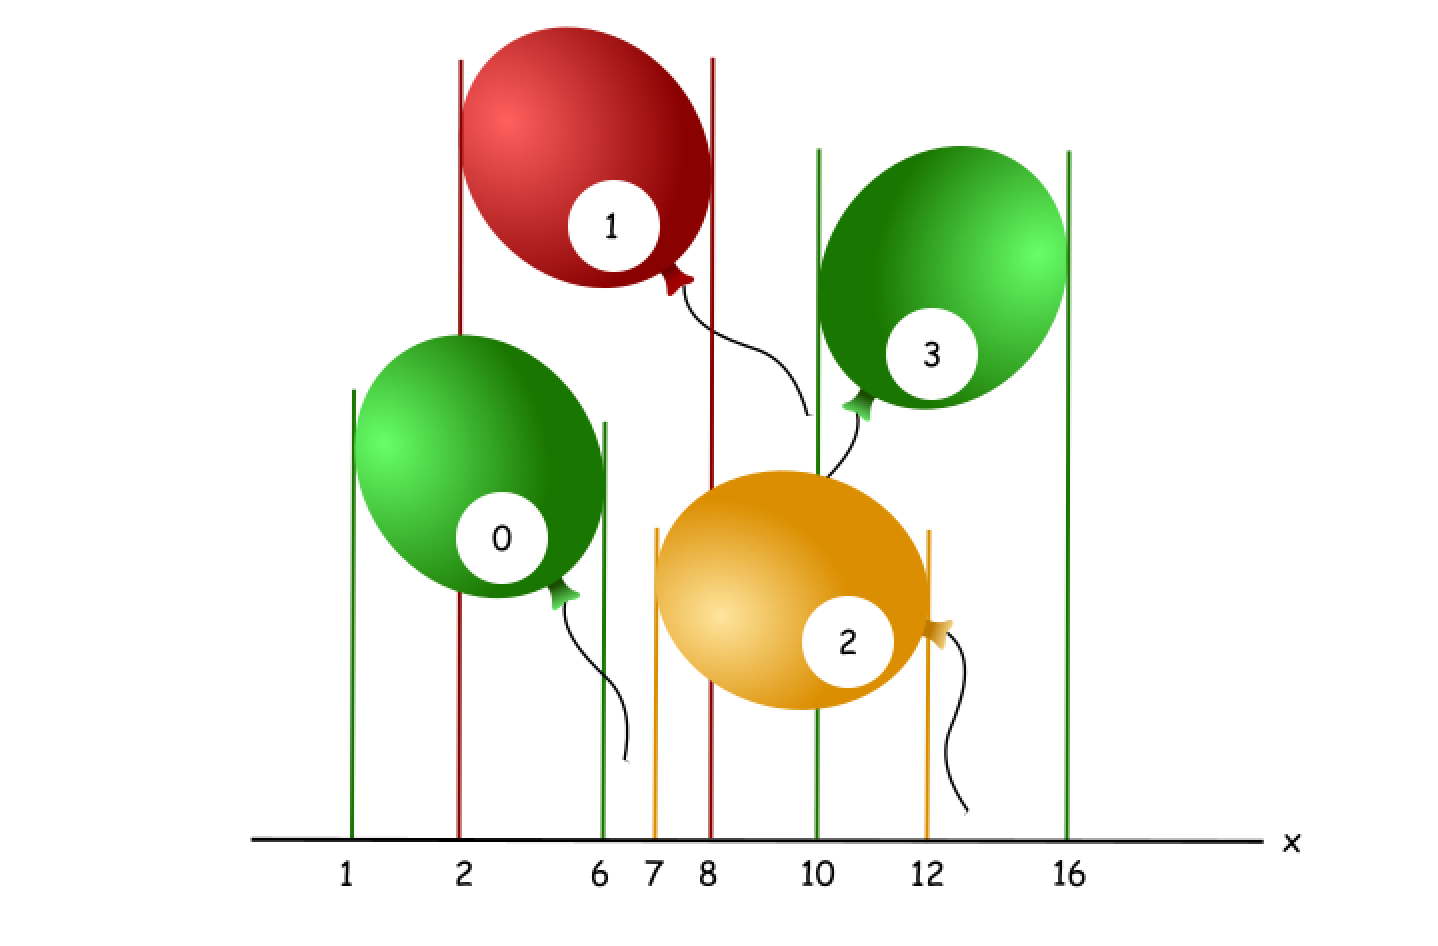
\includegraphics[width=0.5\linewidth]{images/lc0452_eg}
\end{figure}
\item Example 2: {\colorbox{CodeBackground}{\lstinline|points = [[1,2],[3,4],[5,6],[7,8]] --> 4|}}
\item Example 3: {\colorbox{CodeBackground}{\lstinline|points = [[1,2],[2,3],[3,4],[4,5]] --> 2|}}
\end{itemize}

\subsection*{Solution 1 - Greedy, Sort By End}
\begin{enumerate}
\item Sort the balloons by their end points ({\colorbox{CodeBackground}{\lstinline|x_end|}}).
\item Initialize an arrow position at the end point of the first balloon.
\item Iterate through the sorted balloons, and {\color{magenta}{whenever the current balloon starts after the arrow position, increase the number of arrows and set the arrow position to the end point of the current balloon}}.
\end{enumerate}
\begin{lstlisting}
int findMinArrowShots(std::vector<std::vector<int>>& points) {
  std::sort(points.begin(), points.end(),
            [](const std::vector<int>& lhs, const std::vector<int>& rhs) {
              return lhs[1] < rhs[1];
            });
  int num_arrows = 1;
  int arrow_pos = points[0][1];
  for (const std::vector<int>& balloon : points) {
    if (balloon[0] > arrow_pos) {
      ++num_arrows;
      arrow_pos = balloon[1];
    }
  }
  return num_arrows;
}
\end{lstlisting}

\subsection*{*Solution 2 - Greedy, Sort By Start}
\begin{lstlisting}
int findMinArrowShots(std::vector<std::vector<int>>& points) {
  std::sort(points.begin(), points.end(),
            [](const std::vector<int>& lhs, const std::vector<int>& rhs) {
              return lhs[0] < rhs[0];
            });
  int num_arrows = 1;
  int arrow_pos = points[0][1];
  for (const std::vector<int>& balloon : points) {
    if (balloon[0] <= arrow_pos) {
      arrow_pos = std::min(arrow_pos, balloon[1]);
    } else {
      ++num_arrows;
      arrow_pos = balloon[1];
    }
  }
  return num_arrows;
}
\end{lstlisting}

\section{LC 0376 - Wiggle Subsequence}
A \ul{wiggle sequence} is a sequence where the differences between successive numbers \ul{strictly alternate between positive and negative}. A sequence with one element and a sequence with two non-equal elements are trivially wiggle sequences.\\

For example, {\colorbox{CodeBackground}{\lstinline|[1, 7, 4, 9, 2, 5]|}} is a \ul{wiggle sequence} because the differences {\colorbox{CodeBackground}{\lstinline|(6, -3, 5, -7, 3)|}} strictly alternate between positive and negative. In contrast, {\colorbox{CodeBackground}{\lstinline|[1, 4, 7, 2, 5]|}} and {\colorbox{CodeBackground}{\lstinline|[1, 7, 4, 5, 5]|}} are not \ul{wiggle sequences}. The first is not because its first two differences are positive, and the second is not because its last difference is zero.\\

Given an \ul{non-empty} integer array {\colorbox{CodeBackground}{\lstinline|nums|}}, return the length of the \ul{longest wiggle subsequence} of {\colorbox{CodeBackground}{\lstinline|nums|}}.\\

Examples:
\begin{itemize}
\item {\colorbox{CodeBackground}{\lstinline|nums = [1,7,4,9,2,5] --> 6|}}\\
The entire sequence is a wiggle sequence with differences {\colorbox{CodeBackground}{\lstinline|(6, -3, 5, -7, 3)|}}.
\item {\colorbox{CodeBackground}{\lstinline|nums = [1,17,5,10,13,15,10,5,16,8] --> 7|}}\\
There are several subsequences that achieve this length.
One is {\colorbox{CodeBackground}{\lstinline|[1, 17, 10, 13, 10, 16, 8]|}} with differences \newline {\colorbox{CodeBackground}{\lstinline|(16, -7, 3, -3, 6, -8)|}}.
\item {\colorbox{CodeBackground}{\lstinline|nums = [1,2,3,4,5,6,7,8,9] --> 2|}}
\end{itemize}

\subsection*{Solution 1 - Greedy}
\begin{lstlisting}
int wiggleMaxLength(std::vector<int>& nums) {
  int n = nums.size();
  if (n < 2) { return n; }
  int prev_diff = nums[1] - nums[0];
  int max_len = prev_diff == 0 ? 1 : 2;
  for (int i = 2; i < n; ++i) {
    int diff = nums[i] - nums[i - 1];
    if ((prev_diff <= 0 && diff > 0) || (prev_diff >= 0 && diff < 0)) {
      ++max_len;
      prev_diff = diff;
    }
  }
  return max_len;
}
\end{lstlisting}

\subsection*{Solution 2 - Greedy}
\begin{lstlisting}
int wiggleMaxLength(std::vector<int>& nums) {
  int n = nums.size();
  if (n < 2) { return n; }
  // length of the longest wiggle subsequences ending with a rising edge
  int up = 1;
  // length of the longest wiggle subsequences ending with a falling edge
  int down = 1;
  for (int i = 1; i < n; ++i) {
    if (nums[i - 1] < nums[i]) {
      // use rising edge to extend a wiggle subsequence ending with a falling edge
      up = down + 1;
    } else if (nums[i - 1] > nums[i]) {
      // use falling edge to extend a wiggle subsequence ending with a rising edge
      down = up + 1;
    }
  }
  return std::max(up, down);
}
\end{lstlisting}

\section{LC 0763 - Partition Strings without Overlapping Characters}
Given a \ul{non-empty} string {\colorbox{CodeBackground}{\lstinline|s|}}, partition the string into as many parts as possible so that characters in each part don't appear in any other parts. Return a list of integers representing the size of these parts.\\

Examples:
\begin{itemize}
\item {\colorbox{CodeBackground}{\lstinline|s = "ababcbacadefegdehijhklij" --> [9,7,8]|}}\\
The partition is {\colorbox{CodeBackground}{\lstinline|"ababcbaca"|}}, {\colorbox{CodeBackground}{\lstinline|"defegde"|}}, {\colorbox{CodeBackground}{\lstinline|"hijhklij"|}}.\\
This is a partition so that each letter appears in at most one part.\\
A partition like {\colorbox{CodeBackground}{\lstinline|"ababcbacadefegde"|}}, {\colorbox{CodeBackground}{\lstinline|"hijhklij"|}} is incorrect, because it splits s into less parts.
\item {\colorbox{CodeBackground}{\lstinline|s = "eccbbbbdec" --> [10]|}}
\end{itemize}

\subsection*{Solution - Greedy}
\begin{enumerate}
\item First, pass through the string to record the last index of each letter.
\item Next, make another pass through the string to determine the partitions:
  \subitem - Keep track of the current partition's {\colorbox{CodeBackground}{\lstinline|start|}} and {\colorbox{CodeBackground}{\lstinline|end|}}.
  \subitem - {\color{magenta}{For each letter, set the last index of the letters as the end of the current partition.}}
  \subitem - {\color{magenta}{When you reach the end of the partition, record the partition and set the {\colorbox{CodeBackground}{\lstinline|start|}} of the next partition.}}
\end{enumerate}
\begin{lstlisting}
std::vector<int> partitionLabels(std::string s) {
  std::unordered_map<char, int> char2last_idx;
  for (int i = 0; i < s.size(); ++i) { char2last_idx[s[i]] = i; }
  std::vector<int> partitions;
  int start = 0;
  int end = 0;
  for (int i = 0; i < s.size(); ++i) {
    end = std::max(end, char2last_idx[s[i]]);
    if (i == end) {
      partitions.push_back(i - start + 1);
      start = i + 1;
    }
  }
  return partitions;
}
\end{lstlisting}

\section{LC 0738 - Monotone Increasing Digits}
An integer has \ul{monotone increasing digits} if and only if each pair of adjacent digits {\colorbox{CodeBackground}{\lstinline|x|}} and {\colorbox{CodeBackground}{\lstinline|y|}} satisfy {\colorbox{CodeBackground}{\lstinline|x <= y|}}.\\

Given an integer {\colorbox{CodeBackground}{\lstinline|n|}} ({\colorbox{CodeBackground}{\lstinline|n >= 0|}}), return the largest number that is less than or equal to {\colorbox{CodeBackground}{\lstinline|n|}} with \ul{monotone increasing digits}.\\

Examples:
\begin{itemize}
\item {\colorbox{CodeBackground}{\lstinline|n = 10 --> 9|}}
\item {\colorbox{CodeBackground}{\lstinline|n = 1234 --> 1234|}}
\item {\colorbox{CodeBackground}{\lstinline|n = 332 --> 299|}}
\end{itemize}

\subsection*{Solution - Greedy}
Begin with the second digit from the right of {\colorbox{CodeBackground}{\lstinline|num|}} and proceed to the left.  During this process, {\color{magenta}{if you find a digit that violates the monotone increasing rule, decrease the digit}} and set it as {\colorbox{CodeBackground}{\lstinline|marker|}}. After you go through all digits, replace all digits to the right of the {\colorbox{CodeBackground}{\lstinline|marker|}} with {\colorbox{CodeBackground}{\lstinline|9|}}s to maximize the remaining value.

\begin{lstlisting}
int monotoneIncreasingDigits(int num) {
  std::string s = std::to_string(num);
  int n = s.size();
  int marker = n;
  for (int i = n - 2; i >= 0; --i) {
    if (s[i] > s[i + 1]) {
      marker = i;
      s[i] -= 1;
    }
  }
  for (int i = marker + 1; i < n; ++i) { s[i] = '9'; }
  return std::stoi(s);
}
\end{lstlisting}

\section{LC 0968 - Binary Tree Cameras}
You are given the {\colorbox{CodeBackground}{\lstinline|root|}} of a \ul{binary tree}. We install cameras on the tree nodes where each camera at a node can monitor its \ul{parent}, \ul{itself}, and its \ul{immediate children}. Return the minimum number of cameras needed to monitor all nodes of the tree.\\

Examples:
\begin{itemize}
	\item 
	\begin{figure}[H]
		\centering
		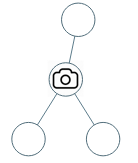
\includegraphics[width=0.15\linewidth]{images/lc0968_example1}
		\label{fig:lc0968example1}
	\end{figure}
	{\colorbox{CodeBackground}{\lstinline|--> 1|}}
	\item 
	\begin{figure}[H]
		\centering
		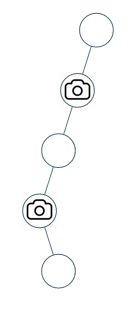
\includegraphics[width=0.15\linewidth]{images/lc0968_example2}
		\label{fig:lc0968example2}
	\end{figure}
	{\colorbox{CodeBackground}{\lstinline|--> 2|}}
\end{itemize}

\subsection*{Solution - Greedy}
TODO